\documentclass[11pt]{article}

\usepackage[margin=1in]{geometry}
\usepackage{amsmath}
\usepackage{booktabs}
\usepackage{array}
\usepackage{tabularx}
\usepackage{graphicx}
\usepackage{float}
\usepackage{caption}
\usepackage{subcaption}
\usepackage{xcolor}
\usepackage{hyperref}
\usepackage{microtype}
\usepackage{listings}

\graphicspath{{../}{./}}
\hypersetup{
  colorlinks=true,
  linkcolor=blue!50!black,
  citecolor=blue!50!black,
  urlcolor=blue!50!black
}
\urlstyle{same}

\lstset{
  basicstyle=\ttfamily\footnotesize,
  breaklines=true,
  frame=single,
  columns=fullflexible,
  keepspaces=true,
  showstringspaces=false,
  tabsize=2
}

\title{\textbf{From Fashion-MNIST to Real-World Clothing Classification}\\
\large Robustness, Transfer Learning, and Human-in-the-Loop Evaluation}
\author{Ashley Cheng}
\date{April 2026}

\begin{document}
\maketitle

\begin{abstract}
Benchmark image datasets make model comparison easy, but they often hide the domain shift that appears in realistic deployment settings. This paper starts with Fashion-MNIST as a controlled multiclass clothing-classification benchmark and then asks whether the same modeling conclusions survive progressively less standardized data. On the clean benchmark, a small convolutional neural network (CNN-small) achieves the strongest performance, reaching a test macro F1 of 0.890 compared with 0.824 for the best classical baseline, PCA plus logistic regression. Under six synthetic perturbations, the CNN remains substantially more robust, with an average macro F1 drop of 0.104 versus 0.431 for the PCA pipeline. An autoencoder-based representation narrows that robustness gap, achieving 0.820 clean macro F1 with a 0.119 average shift penalty. To move beyond grayscale benchmark images, the study then fine-tunes ImageNet-pretrained models on a balanced six-class retail dataset and evaluates the best model on a small personal real-world holdout. A curated ResNet18 reaches 0.917 macro F1 on held-out retail images, but the personal holdout still exposes domain-gap failures caused by crops, context, and taxonomy mismatch. Selective prediction and embedding retrieval show that the strongest deployment setting is not a single hard classifier, but a human-review pipeline that can abstain on uncertain examples and surface visually similar neighbors.
\end{abstract}

\noindent\textbf{Keywords:} image classification, Fashion-MNIST, convolutional neural networks, domain shift, transfer learning, selective prediction, retrieval

\section{Introduction}

Clothing classification is an appealing computer-vision task because it is easy to define but difficult to solve robustly. Controlled datasets such as Fashion-MNIST provide clean labels and standardized images, which makes them well suited for benchmarking \cite{xiao2017fashion}. However, real clothing images rarely look like benchmark data. Product photos vary in color, scale, crop, and background; personal images add clutter, multiple garments, screenshots, and ambiguous examples. As a result, a model that performs well on a clean benchmark may still fail when the image distribution changes.

This paper investigates the following question: \emph{Do image models that outperform classical baselines on Fashion-MNIST remain useful under distribution shift, retail-image fine-tuning, and a small personal real-world holdout?}

To answer that question, the analysis proceeds in stages. First, I compare classical baselines and a small CNN on Fashion-MNIST. Second, I evaluate robustness under synthetic perturbations that mimic archive-like degradation. Third, I test whether learned representations remain useful in two more realistic settings: an unsupervised autoencoder feature pipeline and an ImageNet-pretrained retail transfer-learning pipeline. Finally, I evaluate the best transfer model on a small personal holdout and extend the workflow with selective prediction and embedding retrieval.

The central claim is that \textbf{representation learning matters more as the data become less standardized}. The clean benchmark already favors spatially aware models, but the stronger result is that learned image features degrade more gracefully under shift and adapt more naturally to real-image tasks than flattened-pixel baselines.

\section{Related Work}

Fashion-MNIST was introduced as a more challenging drop-in replacement for MNIST and remains a common benchmark for image-classification experiments \cite{xiao2017fashion}. Classical linear and probabilistic classifiers provide interpretable baselines, but convolutional neural networks are better aligned with the local spatial structure of image data \cite{lecun1998gradient}. When the target domain changes, transfer learning becomes especially valuable because pretrained representations can be adapted with limited labeled data \cite{yosinski2014transferable,russakovsky2015imagenet,he2016resnet,howard2019mobilenetv3}. For deployment, selective classification reframes prediction as a decision about whether to answer or abstain \cite{geifman2017selective}. Learned embeddings can also be reused for retrieval and human review, and modern image-text models suggest a further zero-shot extension \cite{radford2021clip}.

\section{Data and Experimental Design}

\subsection{Controlled Benchmark: Fashion-MNIST}

Fashion-MNIST contains 60,000 training images and 10,000 test images across ten clothing categories \cite{xiao2017fashion}. To keep the experimental pipeline computationally manageable, the supervised benchmark uses a stratified subset of the official training set: 10,000 images for training and 2,000 for validation, with the full official 10,000-image test set reserved for final evaluation. The benchmark remains stratified, so each split preserves class balance.

Each image is a centered $28 \times 28$ grayscale garment. Pixels are rescaled to $[0,1]$. For classical models, each image is flattened to a 784-dimensional vector. For CNNs and the autoencoder, the two-dimensional image structure is retained.

\subsection{Retail Transfer Dataset}

To test transfer beyond Fashion-MNIST, the study uses a curated retail dataset constructed from stable full product images. Because the original ten Fashion-MNIST labels are too granular for noisier retail photos, the real-image task is simplified into six classes: \texttt{top}, \texttt{trouser}, \texttt{dress}, \texttt{outerwear}, \texttt{footwear}, and \texttt{bag}. The resulting dataset contains 720 images total, balanced across classes, with 504 training images, 108 validation images, and 108 test images.

This simplification is methodologically important. It reduces label noise caused by overlapping upper-body classes and partially visible footwear, allowing the experiment to focus on transfer learning rather than on an unstable taxonomy.

\begin{figure}[H]
  \centering
  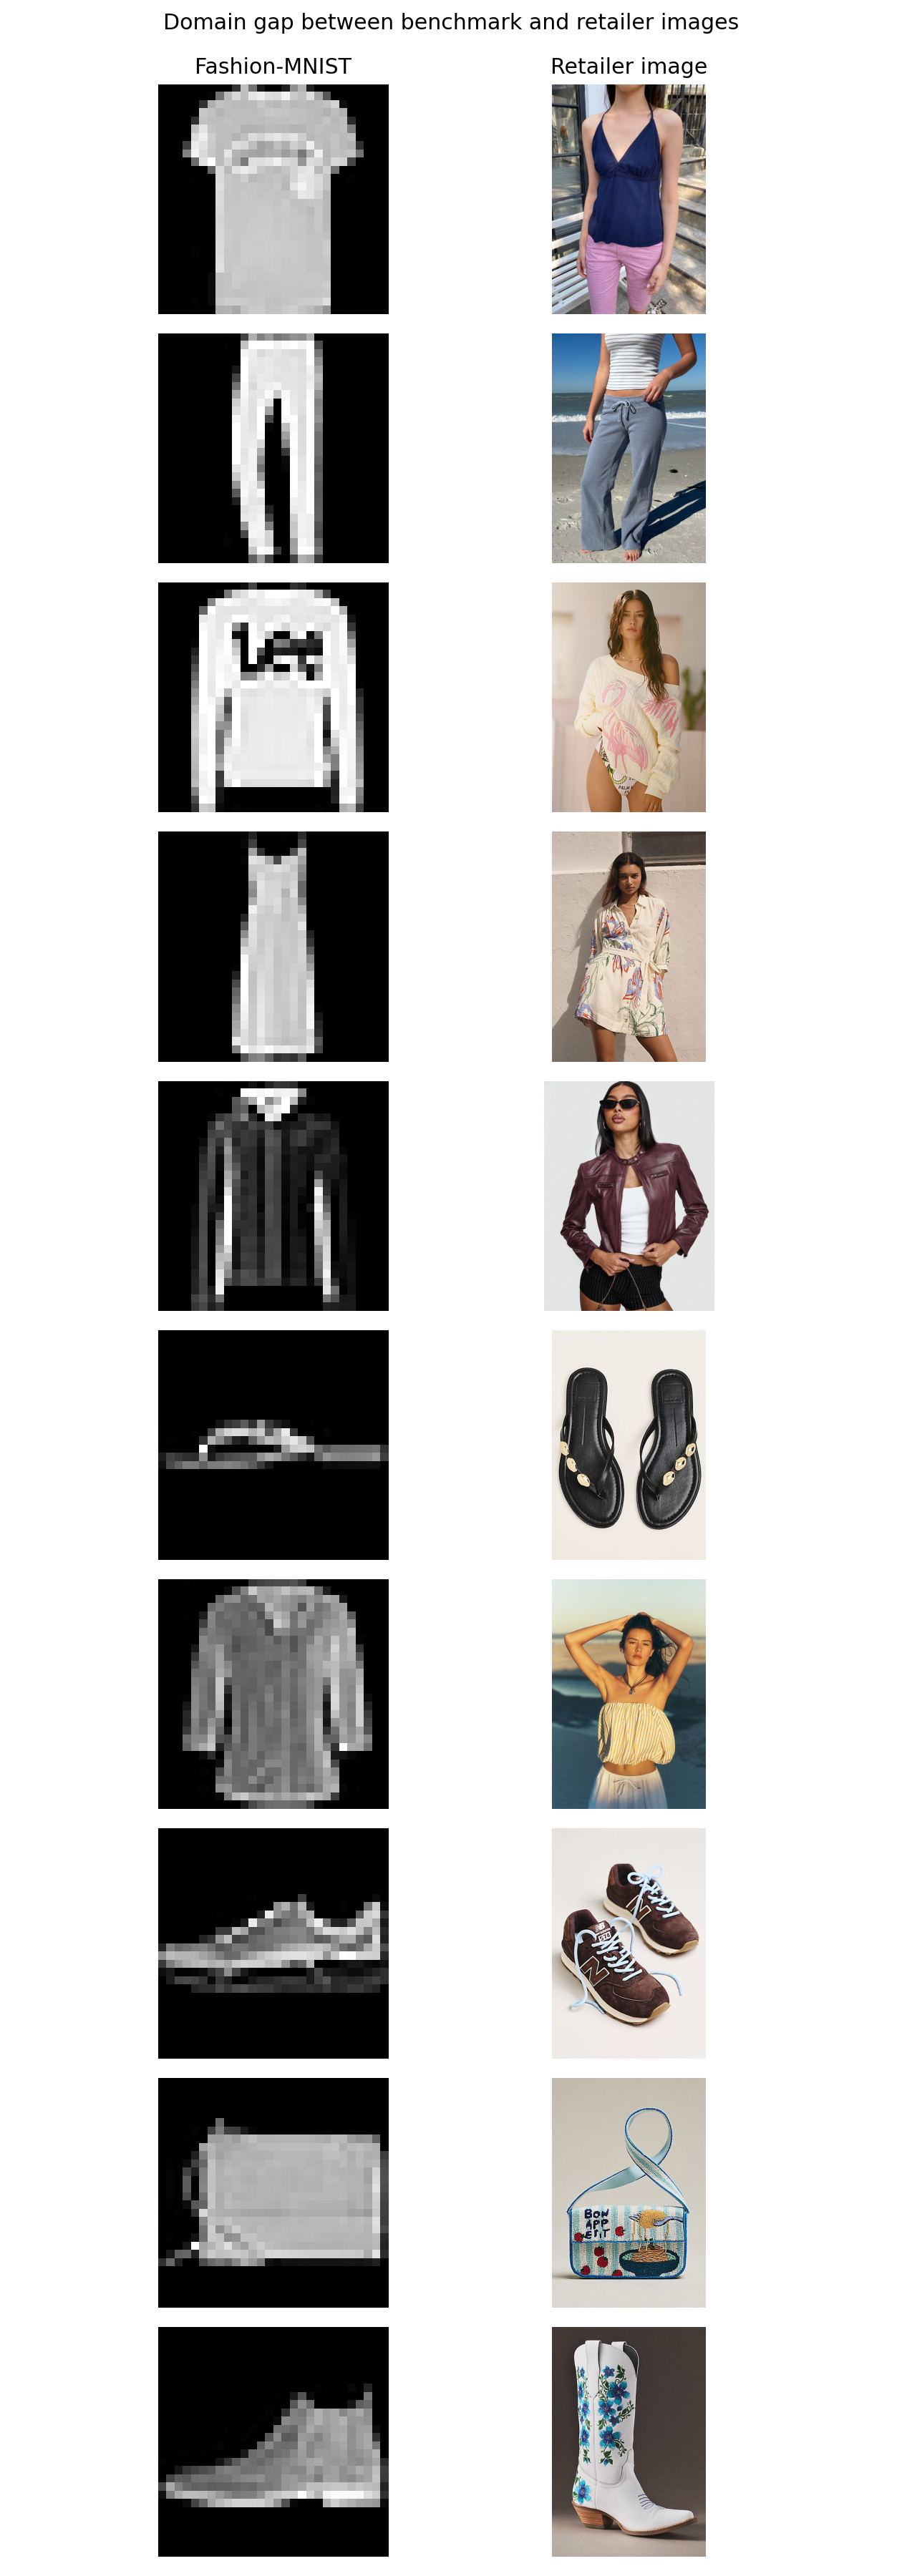
\includegraphics[width=0.92\linewidth,height=0.72\textheight,keepaspectratio]{results/retail_finetune/fashion_vs_retail_examples.png}
  \caption{Domain gap between Fashion-MNIST and raw/full retail product images. Fashion-MNIST is centered, grayscale, and low-resolution. The retail images use the unsegmented full-image pipeline, so the figure avoids the broken segmentation crops that removed parts of some garments.}
  \label{fig:domain_gap}
\end{figure}

\subsection{Segmentation Attempt}

Segmentation was tried as a preprocessing step because, in theory, removing people and backgrounds should make the model focus more directly on the garment. In practice, the segmentation masks were not reliable enough for this dataset. Some outputs removed sleeves, straps, shoe edges, or other class-relevant chunks, and footwear was especially sensitive to those errors. For that reason, the final simplified-label experiment uses raw/full prepared images rather than segmented crops. This keeps background and pose variation in the data, but it avoids training or reporting on visibly broken garment images.

\subsection{Personal Real-World Holdout}

The final stress test uses 11 manually curated personal images drawn from phone photos, screenshots, and archive-like examples. Of these, 10 belong to the six-class retail taxonomy and are scored quantitatively; one is treated as unscored because it is ambiguous or out of vocabulary. This holdout is intentionally too small to serve as a final benchmark. Instead, it functions as a qualitative deployment probe for domain shift.

\subsection{Evaluation Protocol}

The main metric throughout the paper is macro F1, which weights each class equally and is therefore more informative than raw accuracy when comparing heterogeneous error patterns. Accuracy is reported as a secondary metric. For the human-review analysis, I also separate automatic \emph{coverage} from \emph{accepted accuracy}. Given a confidence threshold $\tau$, the set of automatically accepted predictions is
\begin{equation}
A_\tau = \{i : \max_k \hat{p}_{ik} \ge \tau\},
\end{equation}
and scored coverage is
\begin{equation}
\mathrm{coverage}_\tau = \frac{|A_\tau|}{n}.
\end{equation}
This separates model willingness to answer from model correctness on the answers it keeps.

\section{Models}

\subsection{Classical Baselines}

The benchmark begins with four non-image-specific baselines: a majority-class classifier, Gaussian Naive Bayes, multinomial logistic regression, and PCA plus logistic regression. For multiclass logistic regression, the predictive distribution is
\begin{equation}
p(y = k \mid x) = \frac{\exp(w_k^T x + b_k)}{\sum_{j=1}^{K} \exp(w_j^T x + b_j)}.
\end{equation}
These models all consume flattened pixel vectors and therefore ignore the two-dimensional spatial arrangement of the image. PCA is used as a linear compression step before logistic regression; 100 components retain approximately 87.3\% of the training variance.

\subsection{Convolutional and Learned-Feature Models}

The primary image-aware model is a compact CNN trained directly on Fashion-MNIST. The experiments compare two CNN variants and select the smaller model because it achieves the stronger validation macro F1. The best configuration, CNN-small, uses a hidden dimension of 256, dropout of 0.30, learning rate 0.001, and weight decay $10^{-4}$.

To separate representation learning from supervised end-to-end classification, the study also trains an autoencoder on Fashion-MNIST and fits logistic regression on the learned latent vectors. The reconstruction objective is
\begin{equation}
\mathcal{L}_{\mathrm{recon}} = \frac{1}{n} \sum_{i=1}^{n} \|x_i - \hat{x}_i\|_2^2.
\end{equation}
This allows a comparison between linear compression (PCA), unsupervised nonlinear compression (autoencoder), and supervised image features (CNN).

\subsection{Transfer Learning for Retail Images}

The real-image experiment compares ImageNet-pretrained ResNet18 and MobileNetV3-Small backbones. A transfer model can be written as
\begin{equation}
\hat{p}(y=k \mid x) = \mathrm{softmax}(W g_\theta(x) + b)_k,
\end{equation}
where $g_\theta(x)$ is the pretrained visual representation and $(W,b)$ are the learned classification-head parameters. This design starts from broadly useful image features rather than learning from scratch on a small retail dataset.

\section{Results}

\subsection{Clean Fashion-MNIST Benchmark}

Table~\ref{tab:fashion_results} shows a clear hierarchy. Classical models improve substantially over the trivial majority baseline, and PCA plus logistic regression is the strongest classical approach. However, the best overall result comes from CNN-small, which outperforms the best classical pipeline by 0.066 macro-F1 points.

\begin{table}[H]
\centering
\caption{Performance on the clean Fashion-MNIST test set.}
\label{tab:fashion_results}
\begin{tabular}{lrr}
\toprule
Model & Test Accuracy & Test Macro F1 \\
\midrule
Majority class & 0.100 & 0.018 \\
Gaussian Naive Bayes & 0.549 & 0.517 \\
Logistic regression & 0.798 & 0.798 \\
PCA + Logistic regression & 0.826 & 0.824 \\
CNN-small & 0.889 & 0.890 \\
\bottomrule
\end{tabular}
\end{table}

This result supports the expected statistical intuition: preserving spatial locality improves image classification. The remaining confusion is concentrated in visually similar upper-body classes rather than spread uniformly across the label space, which suggests that the CNN has learned meaningful garment structure rather than only memorizing pixel statistics.

\subsection{Robustness Under Synthetic Distribution Shift}

Robustness testing makes the main conclusion stronger. The evaluation perturbs the Fashion-MNIST test set with translations, rotations, blur, noise, brightness and contrast shifts, and crop-plus-pad distortions. Although all models lose performance, the gap between linear and learned representations widens under shift.

\begin{table}[H]
\centering
\caption{Summary of clean performance and average robustness penalty.}
\label{tab:shift_results}
\begin{tabular}{lrr}
\toprule
Model & Clean Test Macro F1 & Avg. Macro F1 Drop \\
\midrule
CNN-small & 0.890 & 0.104 \\
PCA + Logistic regression & 0.824 & 0.431 \\
Autoencoder latent + Logistic regression & 0.820 & 0.119 \\
\bottomrule
\end{tabular}
\end{table}

Two patterns matter. First, the CNN remains the strongest model overall. Second, the autoencoder demonstrates that learned features retain value even without supervised end-to-end training: its clean performance is close to the PCA pipeline, but its robustness is dramatically better. The hardest perturbation for CNN-small is the translation setting, where macro F1 falls to 0.657, yet this remains much more stable than the PCA pipeline under the same family of shifts.

\subsection{Transfer to Curated Retail Images}

The real-image experiment tests whether a benchmark-trained modeling intuition transfers to realistic product imagery. The best fine-tuned model is ResNet18, which reaches a retail test macro F1 of 0.917 on the balanced six-class dataset. This result shows that transfer learning can adapt learned visual representations effectively when the target domain is still relatively clean and class definitions are stabilized.

\begin{table}[H]
\centering
\caption{Held-out retail-image performance on the six-class simplified label space.}
\label{tab:retail_models}
\begin{tabular}{lrr}
\toprule
Model / run & Test Accuracy & Test Macro F1 \\
\midrule
ResNet18, curated & 0.917 & 0.917 \\
ResNet18, full raw simplified split & 0.881 & 0.881 \\
MobileNetV3-Small, curated & 0.833 & 0.835 \\
MobileNetV3-Small, full raw simplified split & 0.802 & 0.804 \\
\bottomrule
\end{tabular}
\end{table}

\begin{figure}[H]
  \centering
  \begin{subfigure}{0.48\linewidth}
    \centering
    
\includegraphics[width=\linewidth]{results/retail_finetune/simplified6_raw_full_resnet18_curated/training_curve.png}
    \caption{Training curve}
  \end{subfigure}
  \hfill
  \begin{subfigure}{0.48\linewidth}
    \centering
    
\includegraphics[width=\linewidth]{results/retail_finetune/simplified6_raw_full_resnet18_curated/confusion_matrix.png}
    \caption{Test confusion matrix}
  \end{subfigure}
  \caption{Curated ResNet18 retail fine-tuning results.}
  \label{fig:retail_training_confusion}
\end{figure}

The retail setup is therefore a useful bridge between benchmark and deployment. It is more realistic than Fashion-MNIST because it includes color images, natural textures, and more varied framing, but it remains cleaner than personal archive-like photos.

\subsection{Personal Holdout and Deployment-Oriented Evaluation}

The personal holdout exposes the remaining domain gap. On the 10 scored images that fit the six-class taxonomy, the fine-tuned ResNet18 achieves 0.700 accuracy and 0.593 macro F1. The drop relative to curated retail performance reflects realistic failure modes: background clutter, close crops, multiple garments, and ambiguous or out-of-taxonomy examples.

\begin{figure}[H]
  \centering
  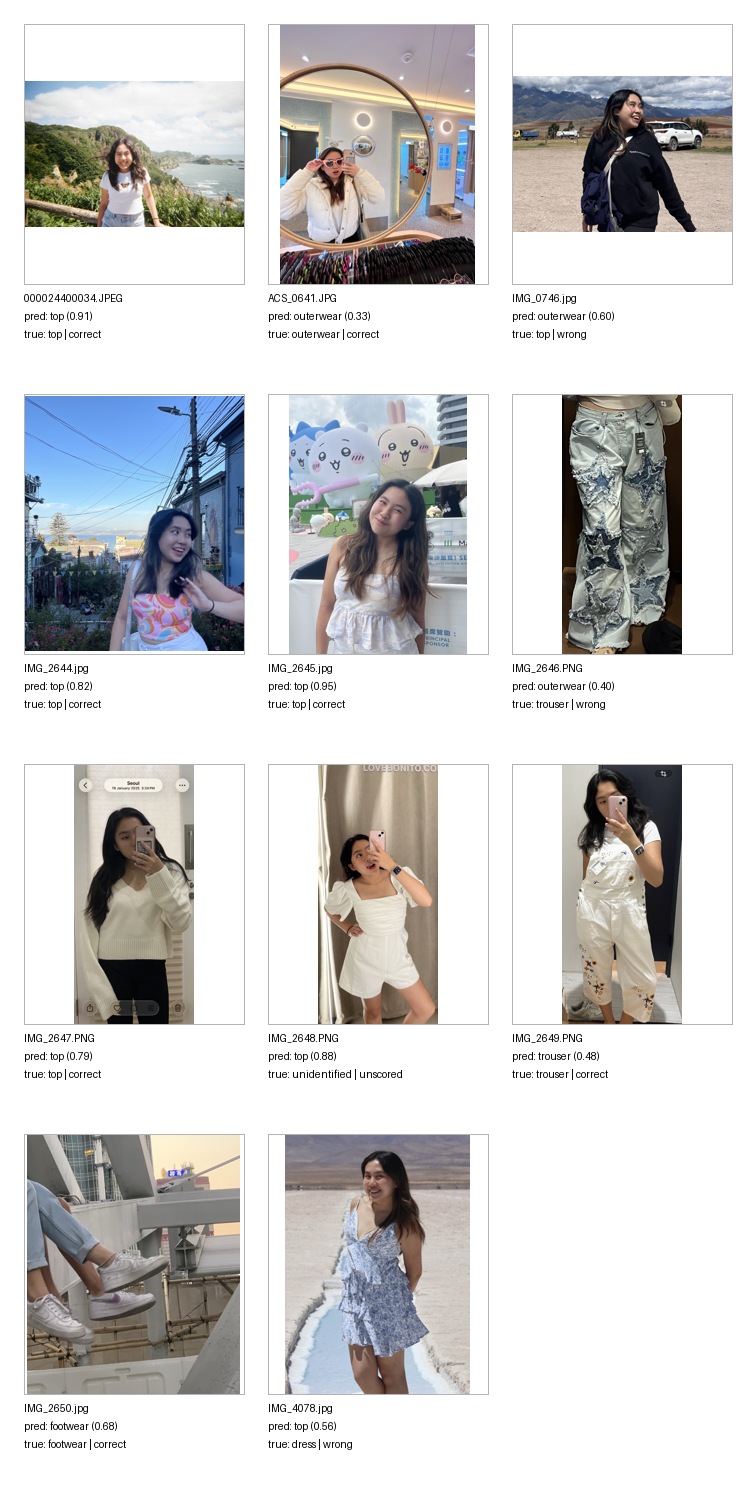
\includegraphics[width=0.85\linewidth,height=0.78\textheight,keepaspectratio]{results/real_world_eval/real_world_predictions.png}
  \caption{Fine-tuned ResNet18 predictions on the personal real-world holdout. The contact sheet shows why this set is better interpreted as a deployment stress test than as a formal benchmark.}
  \label{fig:real_world_predictions}
\end{figure}

Rather than treating these failures as purely negative, the analysis reframes the task in a more deployable way. Table~\ref{tab:deployment_results} summarizes the most useful downstream findings. These numbers suggest that the most realistic use of the system is not fully automated classification. Instead, the learned representation should support a selective, human-in-the-loop workflow: accept only confident predictions, route uncertain cases to review, and use nearest-neighbor retrieval to provide visual context.

\begin{table}[H]
\centering
\caption{Deployment-oriented results on the real-image extensions.}
\label{tab:deployment_results}
\begin{tabularx}{\linewidth}{>{\raggedright\arraybackslash}p{0.29\linewidth}>{\raggedright\arraybackslash}p{0.31\linewidth}>{\raggedright\arraybackslash}X}
\toprule
Setting & Quantitative result & Interpretation \\
\midrule
Curated retail classification & ResNet18 retail test macro F1 = 0.917 & Transfer learning adapts well to a cleaner real-image domain. \\
Personal real-world holdout & Accuracy = 0.700, macro F1 = 0.593 on 10 scored images; 1 additional image left unscored & Domain shift remains substantial once images include personal context and taxonomy mismatches. \\
Selective prediction ($\tau=0.50$) & Coverage = 0.700, accepted accuracy = 0.714 & A modest threshold filters some weak predictions without collapsing automation. \\
Selective prediction ($\tau=0.70$) & Coverage = 0.400, accepted accuracy = 1.000 & Higher confidence thresholds trade throughput for more trustworthy accepted predictions. \\
Selective prediction ($\tau=0.85$) & Coverage = 0.200, accepted accuracy = 1.000 & Very cautious deployment accepts few cases but keeps only high-confidence predictions. \\
Embedding retrieval & Top-1 label match = 0.400; Top-5 contains expected label = 0.900 & Neighbor retrieval is often useful even when single-label classification is brittle. \\
Zero-shot image-text comparison & Zero-shot accuracy = 0.800, macro F1 = 0.648 on the scored subset & Prompt-based classification is promising but needs a larger evaluation set. \\
\bottomrule
\end{tabularx}
\end{table}

\begin{figure}[H]
  \centering
  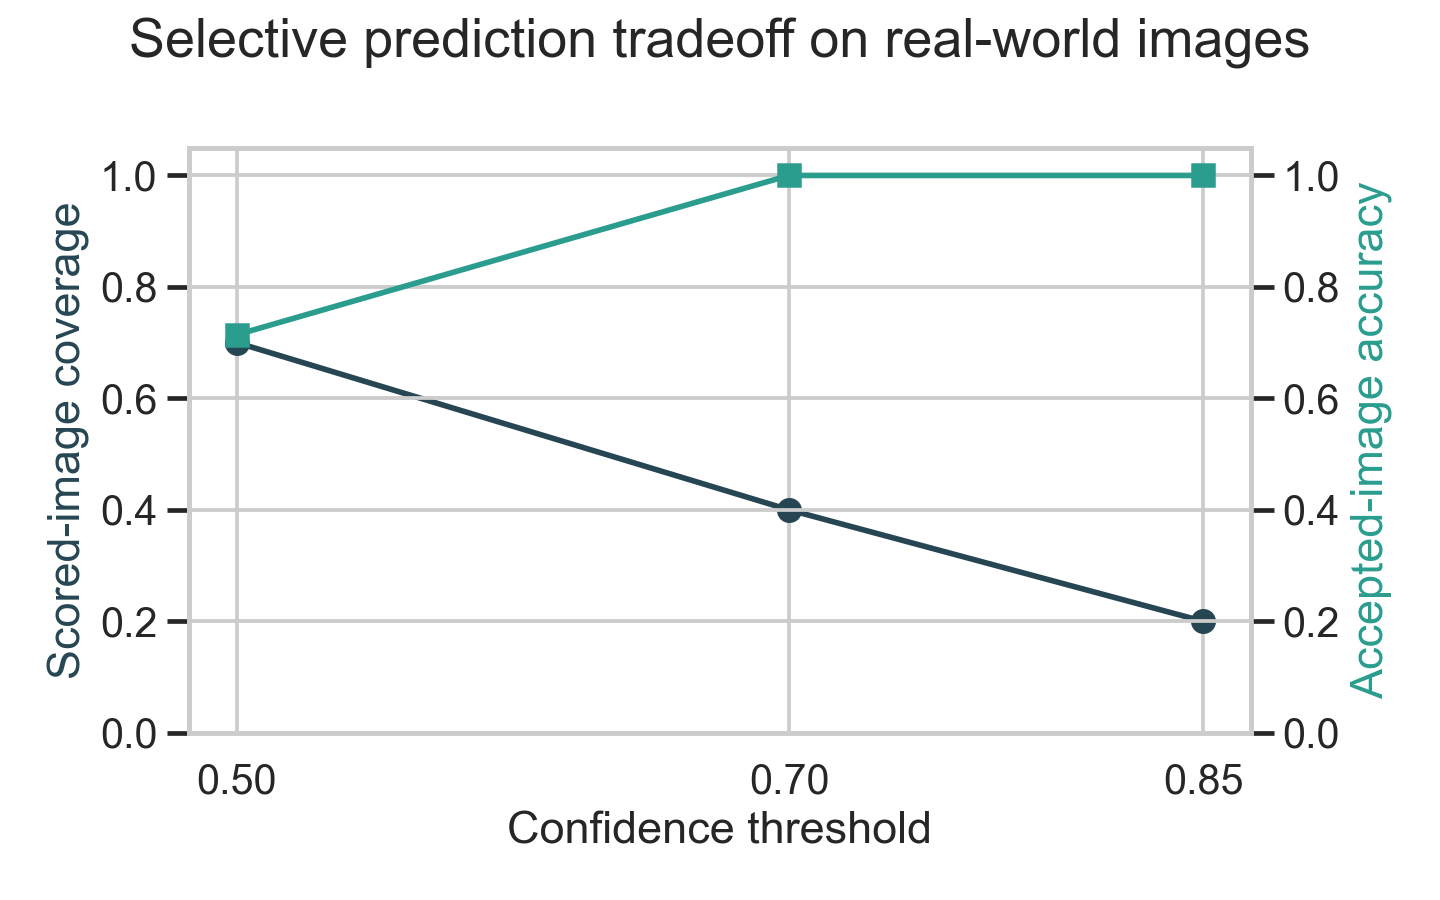
\includegraphics[width=0.78\linewidth]{results/real_world_eval/selective_prediction_tradeoff.png}
  \caption{Coverage and accepted-image accuracy under confidence thresholds. Higher thresholds reduce automation but improve reliability on accepted examples.}
  \label{fig:selective_tradeoff}
\end{figure}

\subsection{Embedding Retrieval and Background Sensitivity}

The fine-tuned ResNet is also useful as an embedding model. Retrieval uses cosine similarity between the real-world query embedding $z_q$ and retail reference embedding $z_r$:
\begin{equation}
s(q,r) = \frac{z_q^T z_r}{\|z_q\|_2 \|z_r\|_2}.
\end{equation}
On the scored personal images, top-1 retrieval matches the expected class for 40\% of examples, but the top-5 neighbors contain the expected class for 90\%. This indicates that retrieval is better treated as a human-review aid than as a direct classifier.

\begin{figure}[H]
  \centering
  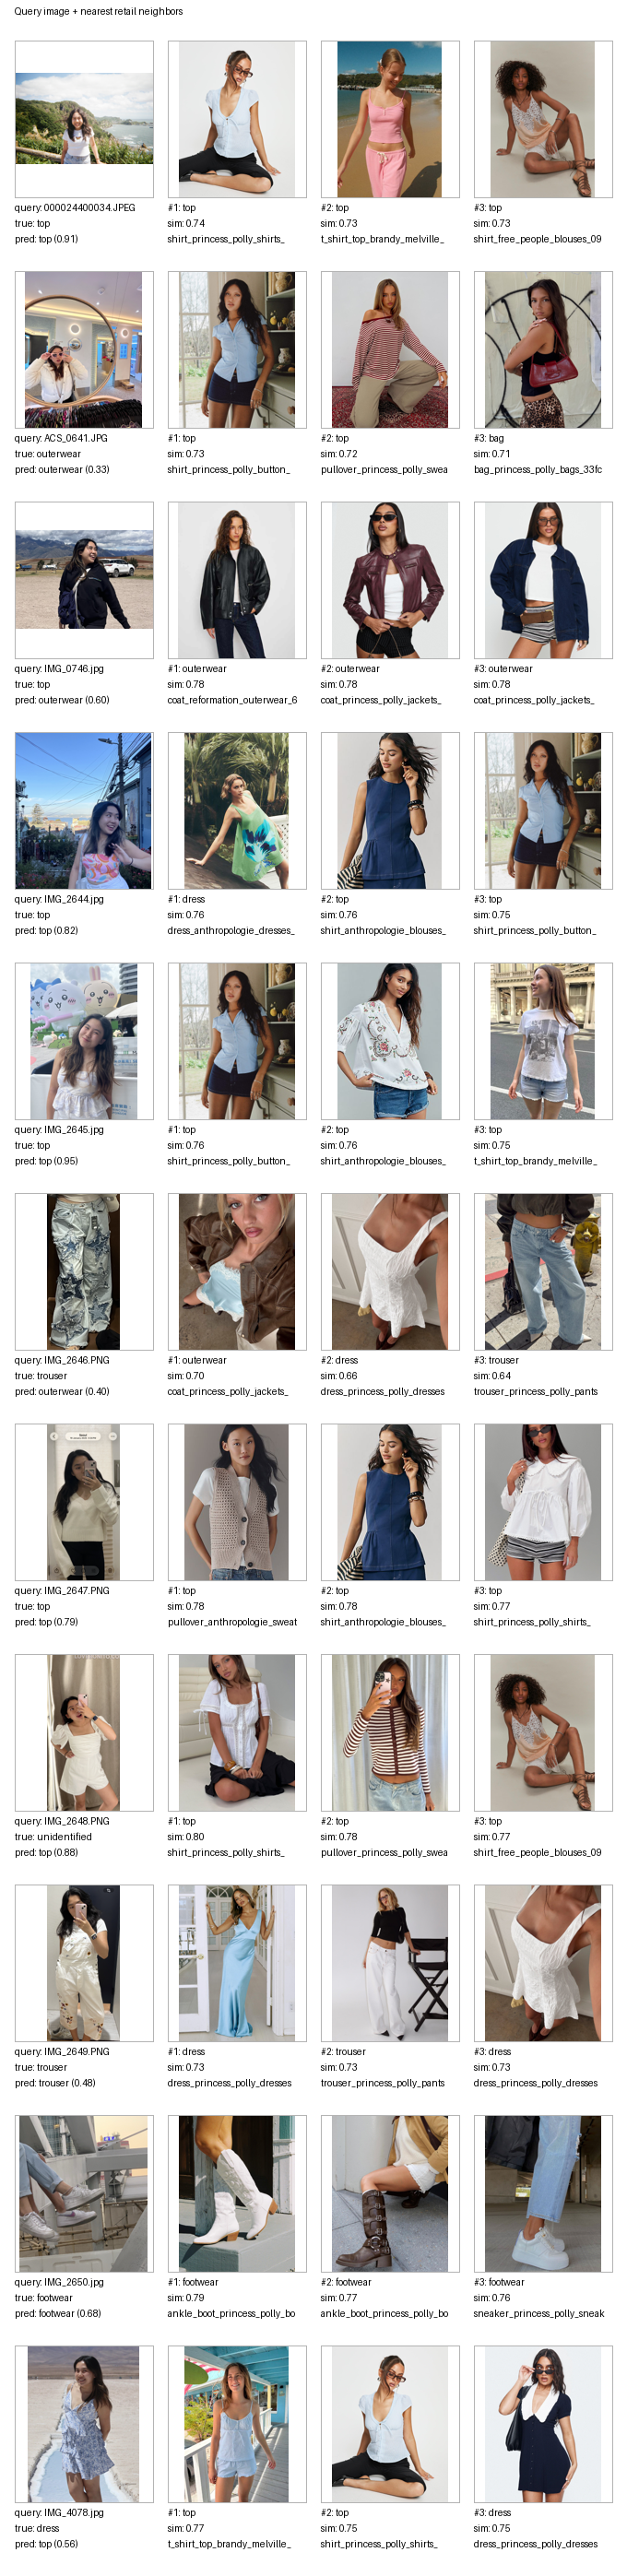
\includegraphics[width=0.9\linewidth,height=0.8\textheight,keepaspectratio]{results/ml_flexibility/retrieval_contact_sheet.png}
  \caption{Nearest-neighbor retrieval from ResNet embeddings. Each query is paired with visually similar retail examples, making model behavior easier to inspect than a single class label.}
  \label{fig:retrieval}
\end{figure}

The retrieval examples also reveal a limitation. The embedding space does not isolate the garment perfectly. Some nearest neighbors appear to share background, pose, color palette, or catalog-photo style rather than only the target clothing item. That does not make retrieval useless; it helps diagnose what the representation is attending to. But it means the retrieved neighbors should be treated as review evidence, not as proof that the ResNet has learned a pure garment-shape representation.

\section{Discussion}

The paper supports a more precise conclusion than simply claiming that CNNs are better than classical baselines. On a clean benchmark, a CNN does outperform flattened-pixel models. More importantly, the advantage grows once the data stop looking perfectly standardized. The robustness results show that representation learning is not only a convenience for clean benchmarks; it changes how gracefully performance degrades under realistic image distortions.

The autoencoder result sharpens that interpretation. Its latent features are not optimized directly for classification, yet they still outperform linear compression under shift. This suggests that nonlinear learned representations capture visual regularities that are useful beyond the exact training distribution. At the same time, the supervised CNN remains best because its features are optimized for the discrimination task itself.

The real-image sections reveal both the promise and the limit of transfer learning. The curated retail results are strong, which indicates that pretrained vision backbones can adapt quickly to a new but related clothing domain. However, the personal holdout shows that deployment-relevant failures remain even when the classification backbone is strong. The most problematic cases are not random errors; they reflect missing taxonomy coverage, context-heavy crops, and examples where multiple garments or outfit-level semantics matter more than a single-item label.

The failed segmentation attempt and the retrieval behavior point to the same deeper issue: the model has not fully separated garment evidence from surrounding visual context. Better object localization might help, but the segmentation experiment also shows that localization can introduce its own errors when masks remove garment parts. A stronger future version would need more robust augmentation, better segmentation quality control, or labels and evaluation metrics that explicitly account for background sensitivity.

\section{Limitations and Future Work}

This study has five main limitations. First, the Fashion-MNIST training subset is deliberately reduced for computational convenience, so the reported benchmark results are strong but not fully optimized. Second, the retail taxonomy is simplified from ten classes to six, which improves stability but reduces granularity. Third, the personal holdout is extremely small and should be interpreted as a deployment probe rather than as a benchmark. Fourth, the main retail figures and final model use raw/full images because segmentation was visually unreliable; this means the model can still learn background, pose, and photography cues. Fifth, the zero-shot image-text extension is conceptually relevant but should be repeated on a larger dataset before drawing strong conclusions.

The most valuable next step is to build a larger labeled personal-image dataset with clearer annotation rules for outfit-level ambiguity. A second improvement would be calibration-aware abstention, not just thresholding on the raw top-class probability. A third would be directly comparing the fine-tuned classifier against zero-shot image-text baselines on a larger and more systematically labeled holdout.

\section{Conclusion}

The results support a simple main finding: image-aware learned representations become more valuable as clothing data become less standardized. On clean Fashion-MNIST, CNN-small outperforms the strongest classical baseline. Under synthetic perturbations, the CNN and the autoencoder-based feature pipeline remain far more stable than PCA plus logistic regression. On curated retail images, transfer learning achieves strong six-class performance, but a small personal holdout still exposes the practical limits of benchmark-to-deployment transfer. The strongest applied takeaway is therefore not a single best classifier, but a review-oriented system that combines representation learning, abstention, and retrieval.

\appendix
\section{Reproducibility Notes}

The paper was generated from the executed notebook \texttt{final.ipynb} and the saved artifacts under \texttt{results/}. The core data and result files used in this paper are:

\begin{itemize}
  \item Curated retail ResNet18 metrics and class report in the \path{simplified6_raw_full_resnet18_curated} result folder
  \item \path{results/real_world_eval/predictions.csv}
  \item \path{results/real_world_eval/selective_prediction_summary.csv}
  \item \path{results/ml_flexibility/retrieval_summary.csv}
  \item \path{results/ml_flexibility/zero_shot_comparison.csv}
\end{itemize}

\section{Pipeline Commands}

\begin{lstlisting}[language=bash,caption={Retail-image extension commands.}]
python scripts/scrape_retail_images.py
python scripts/segment_retail_images.py
python scripts/validate_retail_dataset.py
python scripts/make_retail_eda.py --validated data/retail_images/metadata/validated_raw_images.csv
python scripts/make_simplified6_retail_splits.py
python scripts/train_retail_finetune.py \
  --label-column simplified_class \
  --model resnet18
\end{lstlisting}

\section{Segmentation and Background Sensitivity}

Segmentation was kept as an audit trail rather than as the main preprocessing policy. The segmented outputs are stored under \path{data/retail_images/segmented/}, with quality overlays under \path{data/retail_images/segmentation_overlays/}. Visual inspection showed that segmentation sometimes removed class-relevant garment parts. Because of that, the final EDA figure and the six-class retail splits use raw/full images from \path{validated_raw_images.csv} and \path{splits_raw_full_simplified6.csv}.

This decision creates a tradeoff. Raw/full images avoid broken crops, but they leave the model exposed to background and styling cues. The retrieval experiment makes that limitation visible: nearest neighbors are often useful, and the expected class appears somewhere in the top five for most scored queries, but top-one neighbors sometimes appear to match pose, context, color, or catalog style more than the exact target garment. Methodologically, this is useful evidence because preprocessing choices can move the error from one place to another rather than simply solving it.

\section{Representative Evaluation Code}

\begin{lstlisting}[language=Python,caption={Metric helper used throughout the notebook.}]
def evaluate_predictions(y_true, y_pred):
    return {
        "accuracy": accuracy_score(y_true, y_pred),
        "macro_f1": f1_score(y_true, y_pred, average="macro"),
    }
\end{lstlisting}

\begin{lstlisting}[language=Python,caption={Selective prediction policy.}]
accepted = predictions[predictions["top1_confidence"] >= threshold]
reviewed = predictions[predictions["top1_confidence"] < threshold]

coverage = len(accepted) / len(predictions)
accepted_accuracy = accuracy_score(
    accepted["expected_simplified_class"],
    accepted["predicted_class"],
)
\end{lstlisting}

\begin{thebibliography}{9}

\bibitem{xiao2017fashion}
Han Xiao, Kashif Rasul, and Roland Vollgraf.
\newblock Fashion-MNIST: A Novel Image Dataset for Benchmarking Machine Learning Algorithms.
\newblock \emph{arXiv:1708.07747}, 2017.

\bibitem{lecun1998gradient}
Yann LeCun, Leon Bottou, Yoshua Bengio, and Patrick Haffner.
\newblock Gradient-Based Learning Applied to Document Recognition.
\newblock \emph{Proceedings of the IEEE}, 86(11):2278--2324, 1998.

\bibitem{yosinski2014transferable}
Jason Yosinski, Jeff Clune, Yoshua Bengio, and Hod Lipson.
\newblock How Transferable Are Features in Deep Neural Networks?
\newblock \emph{Advances in Neural Information Processing Systems}, 2014.

\bibitem{russakovsky2015imagenet}
Olga Russakovsky et al.
\newblock ImageNet Large Scale Visual Recognition Challenge.
\newblock \emph{International Journal of Computer Vision}, 115:211--252, 2015.

\bibitem{he2016resnet}
Kaiming He, Xiangyu Zhang, Shaoqing Ren, and Jian Sun.
\newblock Deep Residual Learning for Image Recognition.
\newblock \emph{Proceedings of the IEEE Conference on Computer Vision and Pattern Recognition}, 2016.

\bibitem{howard2019mobilenetv3}
Andrew Howard et al.
\newblock Searching for MobileNetV3.
\newblock \emph{Proceedings of the IEEE/CVF International Conference on Computer Vision}, 2019.

\bibitem{geifman2017selective}
Yonatan Geifman and Ran El-Yaniv.
\newblock Selective Classification for Deep Neural Networks.
\newblock \emph{Advances in Neural Information Processing Systems Workshops}, 2017.

\bibitem{radford2021clip}
Alec Radford et al.
\newblock Learning Transferable Visual Models From Natural Language Supervision.
\newblock \emph{International Conference on Machine Learning}, 2021.

\end{thebibliography}

\end{document}
